% !TEX root=./whitepaper.tex
\section{Key-Value Runtime}

\projabbrev Storage provides a Key-Value runtime upon the log layer. 
Each key-value node can access the key-value store state through the runtime interface. 
The key-value runtime provides the standard interface like \texttt{Put()} and \texttt{Get()}, and accepts serialized key-value pair from any application-specific structure. 

During the normal execution of the key-value store node, it maintains the latest key-value state locally. It updates the value of a key through \texttt{Put()} API which composes a log entry containing the updated key-value pair and appends to the log. 
The runtime constantly monitors the new log entries in the log and fetches them back to the key-value node and updates the local key-value state according to the log entry contents. 
In this sense, multiple key-value store nodes essentially synchronize with each other through the shared decentralized log.
A user-defined function will be used to deserialize the raw content in the log entry to the application-specific key-value structure.
Application can use \texttt{Get()} API to access the latest value of a given key. 
To improve the efficiency of the updates for small key-value pairs, the \texttt{Put()} allows batched updates with multiple key-value pairs at once. 
Figure~\ref{fig:kv} illustrates the architecture of the decentralized key-value store. 
To manage the access control, the ownership information of each key can also be maintained in the log entries.
All the honest key-value nodes follow the same update rule for the keys based on the ownership to achieve the state consistency.

\begin{figure}[H]	
	%\vspace{-6mm}
	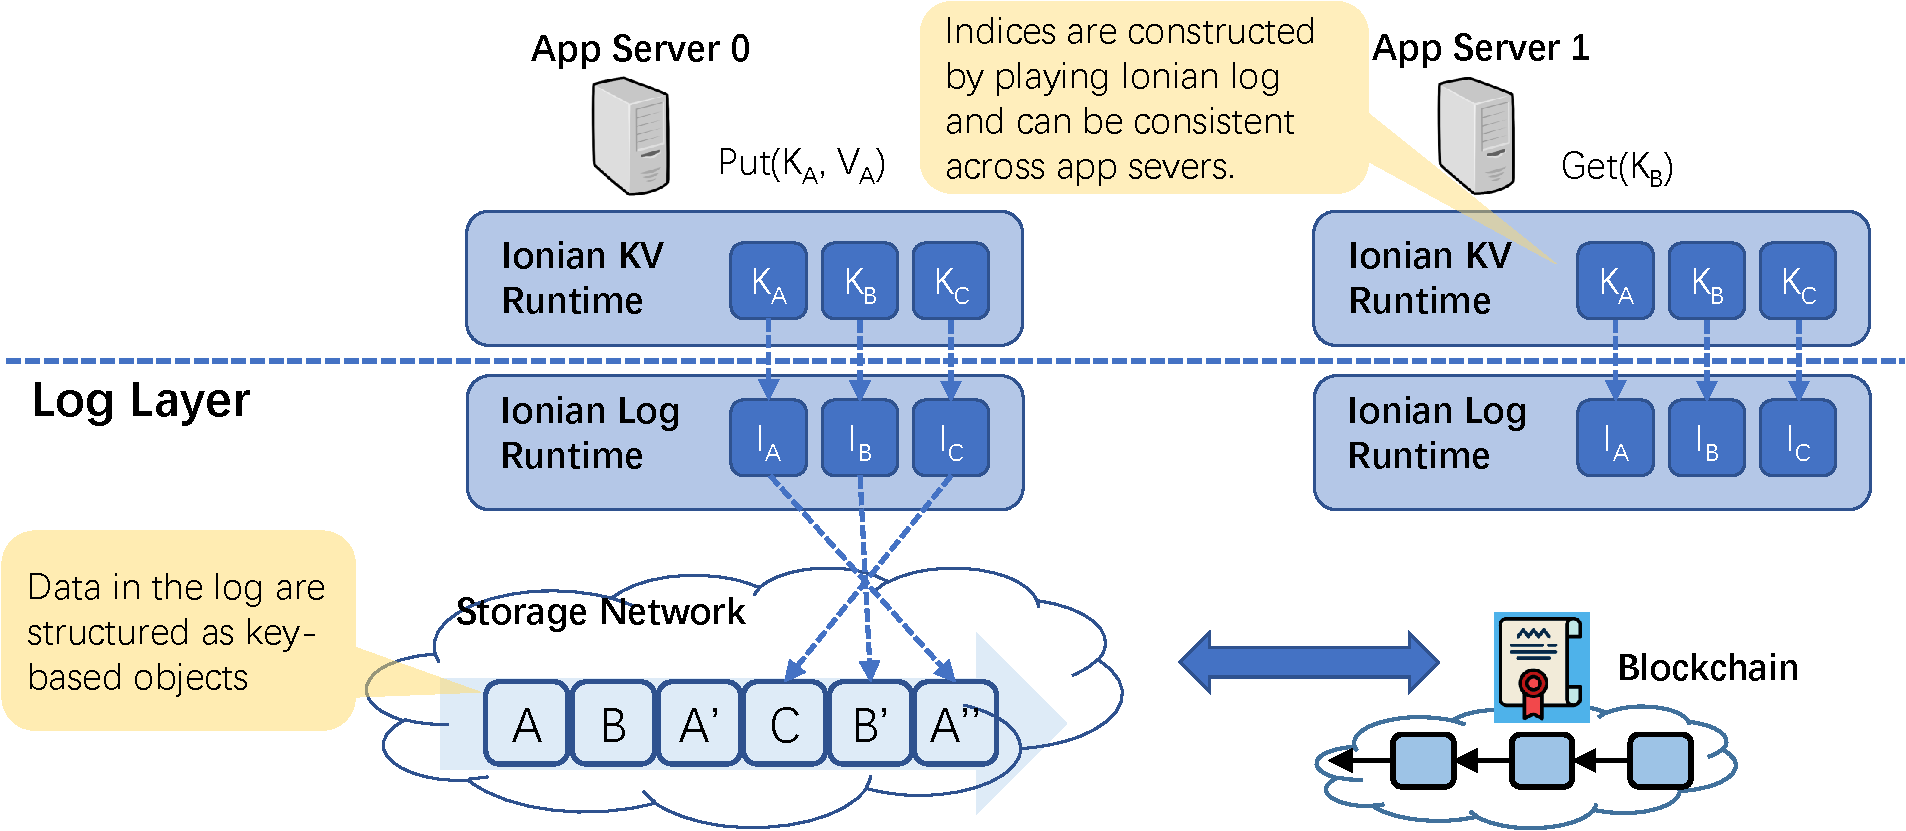
\includegraphics[width=\textwidth]{figure/kv-crop.pdf}
	\caption{Decentralized Key-Value Store}
	\label{fig:kv}
	%\vspace{-10mm}
\end{figure}

When a new key-value node just joins the network, it connects to the log layer and plays the log entries from head to tail to construct the latest state of the key-value store.
During the log entry playing, an application-specific key-value node can skip irrelevant log entries which do not contain the stream IDs that it cares.
